% !TEX root =  master.tex
\chapter{Einleitung}
Die IT-Sicherheit wird zunehmend wichtiger im Privaten- und im Unternehmenssektor. Das Erkennen von Sicherheitslücken und deren Schließung ist die Aufgabe der IT-Sicherheit. Diese in 3 Phasen gegliederte Projektarbeit zeigt Methoden, um diese Sicherheitslücken zu erkennen und gegebenenfalls Maßnahmen dafür zu ergreifen. Für die Dokumentation wurde Kali Linux verwendet und der Ablauf durch Beschreibung von Screenshots erläutert. Es wurden virtuelle Maschinen lokal und auch extern genutzt.
\begin{figure}
    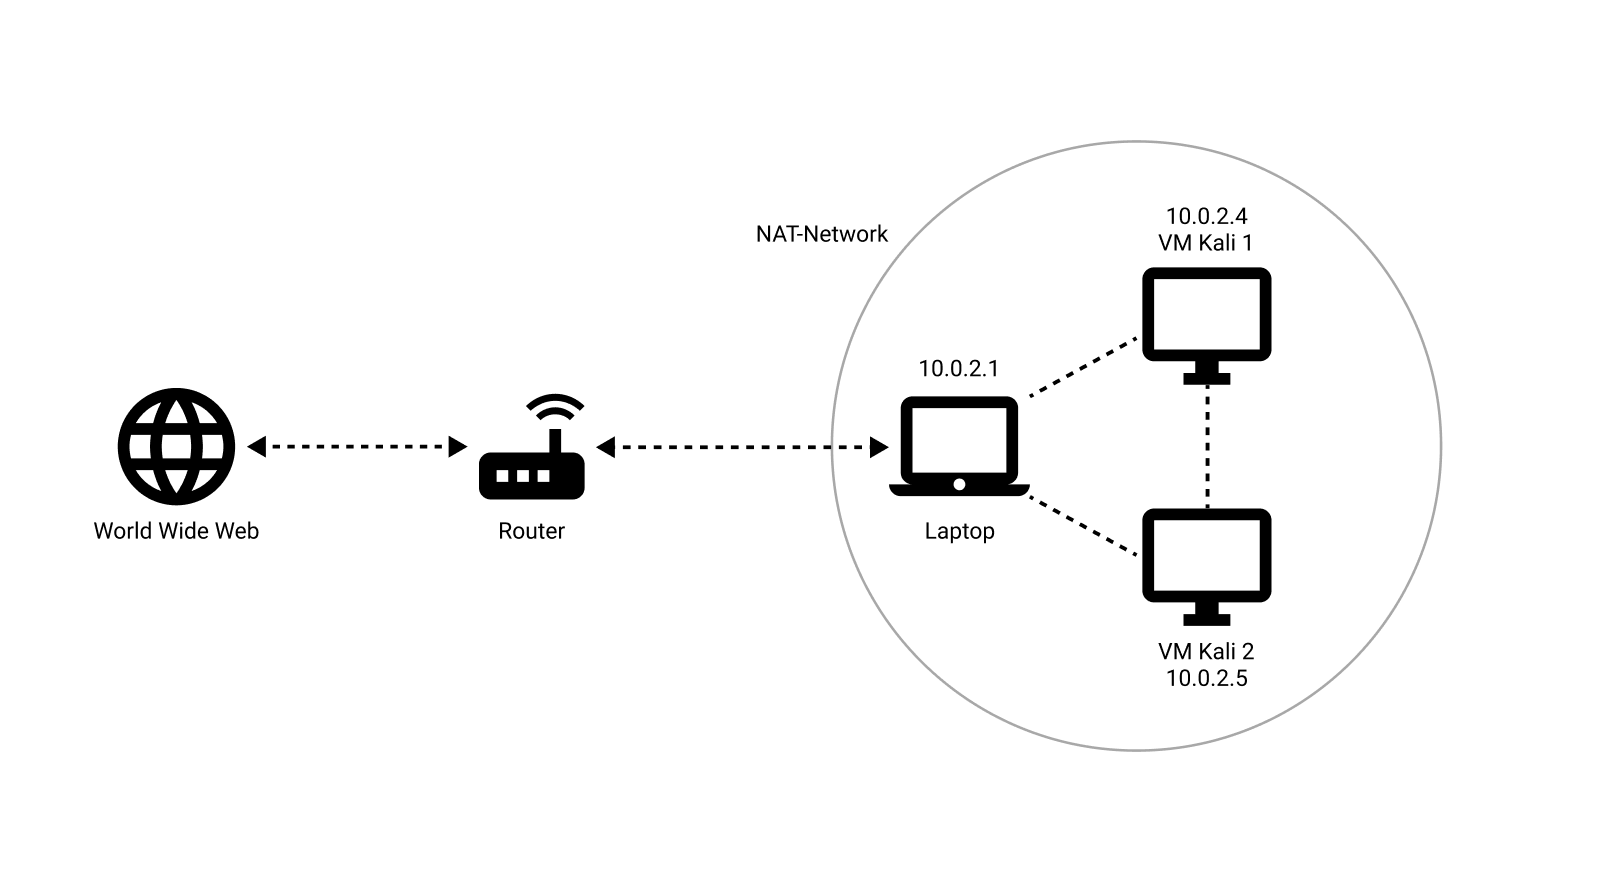
\includegraphics[width=\linewidth]{img/network_fig.png}
    \caption{Aufbau des Netzwerks}
    \label{fig:network}
\end{figure}
\section*{Maybe Project preview or smth…}
